%!TEX root = ../template.tex
%%%%%%%%%%%%%%%%%%%%%%%%%%%%%%%%%%%%%%%%%%%%%%%%%%%%%%%%%%%%%%%%%%%%
%% chapter7.tex
%% NOVA thesis document file
%%
%% Chapter with lots of dummy text
%%%%%%%%%%%%%%%%%%%%%%%%%%%%%%%%%%%%%%%%%%%%%%%%%%%%%%%%%%%%%%%%%%%%

\typeout{NT FILE chapter7.tex}%

\chapter{Red-Black Ant Colony System}
\label{chapt:6}

\section{Introduzione}

Questo capitolo presenta una versione modificata dell'algoritmo \gls{ACS}, chiamata Red-Black Ant Colony System (\gls{RB-ACS}), che mira a migliorare le prestazioni dell'\gls{ACS} su istanze di grandi dimensioni del \gls{TSP}. Il \gls{RB-ACS} incorpora diverse migliorie chiave all'approccio  \gls{ACS} standard, tra cui la ricerca in parallelo, l'inizializzazione migliorata dei feromoni e l'impostazione di parametri differenziati per i due gruppi di formiche. Queste modifiche sono progettate per consentire al \gls{RB-ACS} di esplorare lo spazio di ricerca in modo più efficace e di convergere efficientemente verso soluzioni ottimali o quasi-ottimali, anche per problemi di \gls{TSP} su larga scala \cite{Hassan2013}.

\section{L'Algoritmo Red-Black Ant Colony System (\gls{RB-ACS})}
Mentre l'algoritmo  \gls{ACS} standard si è dimostrato efficace nella risoluzione di istanze del \gls{TSP}, le sue prestazioni possono peggiorare all'aumentare delle dimensioni del problema. Il Red-Black Ant Colony System (\gls{RB-ACS})  introduce diverse modifiche chiave all'approccio  \gls{ACS} standard per migliorarne la scalabilità e la qualità delle soluzioni per problemi di \gls{TSP} su larga scala \cite{Hassan2013}.

\begin{figure}[h!]
  \centering
  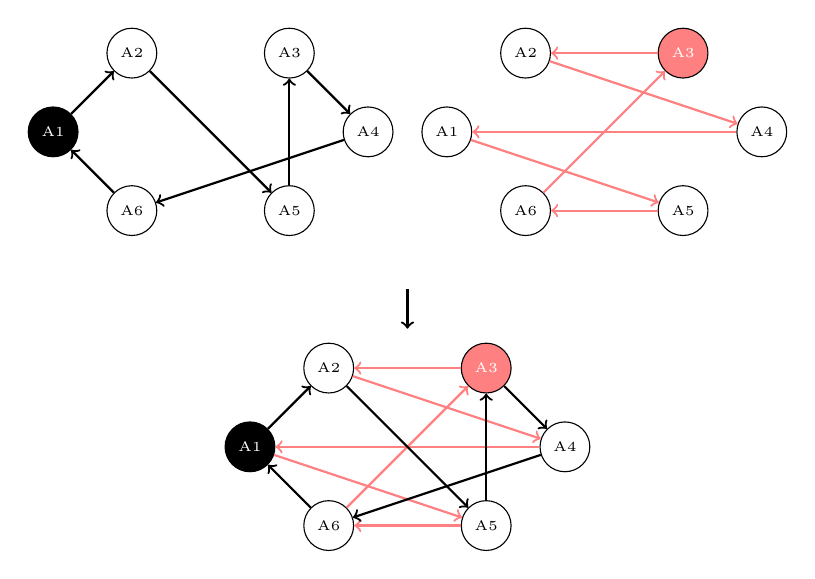
\begin{tikzpicture}[node distance=1.5cm]
    % Left diagram
    \node[circle,draw, fill=black, text=white] (A1) at (-2,0) {\tiny A1};
    \node[circle,draw] (A2) at (-1,1) {\tiny A2};
    \node[circle,draw] (A3) at (1,1) {\tiny A3};
    \node[circle,draw] (A4) at (2,0) {\tiny A4};
    \node[circle,draw] (A5) at (1,-1) {\tiny A5};
    \node[circle, draw] (A6) at (-1, -1) {\tiny A6};
    
    \draw[->,thick] (A1) -- (A2);
    \draw[->,thick] (A2) -- (A5);
    \draw[->,thick] (A5) -- (A3);
    \draw[->,thick] (A3) -- (A4);
    \draw[->, thick] (A6) -- (A1);
    \draw[->, thick] (A4) -- (A6);

    % Right diagram

    \node[circle,draw] (A1) at (-2 + 5,0) {\tiny A1};
    \node[circle,draw] (A2) at (-1 + 5,1) {\tiny A2};
    \node[circle,draw, fill=red!50, text = white] (A3) at (1+5,1) {\tiny A3};
    \node[circle,draw] (A4) at (2+5,0) {\tiny A4};
    \node[circle,draw] (A5) at (1+5,-1) {\tiny A5};
    \node[circle, draw] (A6) at (-1+5, -1) {\tiny A6};
    
    \draw[->,thick, color = red!50] (A3) -- (A2);
    \draw[->,thick, color = red!50] (A2) -- (A4);
    \draw[->,thick, color = red!50] (A4) -- (A1);
    \draw[->,thick, color = red!50] (A1) -- (A5);
    \draw[->, thick, color = red!50] (A5) -- (A6);
    \draw[->, thick, color = red!50] (A6) -- (A3);


        % Connecting arrow
    \draw[->, thick] (2.5,-2) -- (2.5,-2.5);

    \node[circle,draw, fill=black, text=white] (A1) at (-2+2.5,0-4) {\tiny A1};
    \node[circle,draw] (A2) at (-1+2.5,1-4) {\tiny A2};
    \node[circle,draw, fill=red!50, text=white] (A3) at (1+2.5,1-4) {\tiny A3};
    \node[circle,draw] (A4) at (2+2.5,0-4) {\tiny A4};
    \node[circle,draw] (A5) at (1+2.5,-1-4) {\tiny A5};
    \node[circle, draw] (A6) at (-1+2.5, -1-4) {\tiny A6};
     
    \draw[->,thick, color = red!50] (A3) -- (A2);
    \draw[->,thick, color = red!50] (A2) -- (A4);
    \draw[->,thick, color = red!50] (A4) -- (A1);
    \draw[->,thick, color = red!50] (A1) -- (A5);
    \draw[->, thick, color = red!50] (A5) -- (A6);
    \draw[->, thick, color = red!50] (A6) -- (A3);
 
    \draw[->,thick] (A1) -- (A2);
    \draw[->,thick] (A2) -- (A5);
    \draw[->,thick] (A5) -- (A3);
    \draw[->,thick] (A3) -- (A4);
    \draw[->, thick] (A6) -- (A1);
    \draw[->, thick] (A4) -- (A6);
\end{tikzpicture}
  \caption{}\label{fig:}
\end{figure}


\subsection{Inizializzazione dei Feromoni}
Nell' \gls{ACS} standard, il livello iniziale di feromone su tutti i archi è impostato a un valore costante $\tau_0$. Nel \gls{RB-ACS}, gli autori propongono uno schema di inizializzazione dei feromoni diverso, in cui il livello iniziale di feromone su ciascun bordo $(r,s)$ è impostato secondo la seguente equazione:
\begin{equation}
	\tau_\text{init}(r,s) = \frac{C}{\text{costo}(r,s)}
\end{equation}
dove $C$ è una costante e $\text{costo}(r,s)$ è la distanza tra le città $r$ e $s$. Questa inizializzazione modificata dei feromoni incoraggia le formiche a esplorare i archi più corti, che sono più desiderabili per il tour ottimale, assegnando loro livelli di feromone iniziali più alti \cite{Hassan2013}.

\subsection{Ricerca in Parallelo con Gruppi di Formiche Rosse e Nere}
Un'altra modifica chiave nell'algoritmo \gls{RB-ACS} è l'utilizzo di due gruppi separati di formiche, chiamati "rosse" e "nere", che esplorano lo spazio di ricerca in parallelo. Nell'\gls{ACS} standard, un singolo gruppo di formiche costruisce i tour e le formiche possono seguire i percorsi di altre formiche, il che può portare a una convergenza prematura e a rimanere bloccati in minimi locali.

Nel \gls{RB-ACS}, i gruppi di formiche rosse e nere operano in modo indipendente, mantenendo ciascuno i propri sentieri di feromoni e cercando soluzioni senza essere influenzati dall'altro gruppo. Questo approccio di ricerca parallela riduce la probabilità che l'algoritmo rimanga bloccato in minimi locali, poiché i due gruppi di formiche possono esplorare regioni diverse dello spazio di ricerca simultaneamente \cite{Hassan2013}.

\subsection{Impostazioni di Parametri Differenziate}
Oltre al processo di ricerca separato, l'algoritmo \gls{RB-ACS} impiega anche diverse impostazioni dei parametri per i gruppi di formiche rosse e nere. In particolare, la regola di aggiornamento locale dei feromoni e il tasso di evaporazione dei feromoni possono essere impostati su valori diversi per i due gruppi. Questa differenziazione è ispirata al comportamento osservato delle formiche reali, in cui colonie o gruppi diversi possono presentare caratteristiche distinte, come i tassi di deposizione e di evaporazione dei feromoni \cite{Hassan2013}.

Utilizzando impostazioni di parametri separate per le formiche rosse e nere, l'algoritmo \gls{RB-ACS} può ulteriormente migliorare la diversificazione del processo di ricerca, permettendo ai due gruppi di esplorare lo spazio di soluzione in modo più complementare.

\subsection{Aggiornamento Globale dei Feromoni Migliorato}
Nell' \gls{ACS} standard, solo la formica globalmente migliore è autorizzata a depositare feromoni durante la fase di aggiornamento globale. Nel \gls{RB-ACS}, gli autori propongono una regola di aggiornamento globale modificata, in cui le due migliori formiche di ciascuno dei gruppi rosso e nero sono autorizzate ad aggiornare i livelli di feromone. Questo aggiornamento globale parallelo rafforza ulteriormente la ricerca verso soluzioni di alta qualità, poiché vengono rinforzati simultaneamente diversi percorsi promettenti \cite{Hassan2013}.

\subsection{Pseudocodice}

% TODO: Inserire il pseudocodice dell'algoritmo \gls{RB-ACS}
\begin{algorithm}
	\caption{Red-Black Ant Colony System (\gls{RB-ACS}) per il \gls{TSP}}
	\begin{algorithmic}[1]
		\State Inizializza i livelli di feromoni $\tau_{ij} = \tau_{\text{init}}(i,j)$ per tutti gli archi $(i,j)$
		\State Inizializza la migliore soluzione globale $S_{gb}$ e la sua lunghezza $L_{gb}$
		\For{ogni iterazione}
		\For{ogni gruppo di formiche $g \in \{\text{rosso}, \text{nero}\}$}
		\For{ogni formica $k = 1, \ldots, m_g$}
		\State Posiziona la formica $k$ del gruppo $g$ su una città di partenza casuale
		\State Inizializza il tour parziale $S_k^g = \emptyset$
		\Repeat
		\State Seleziona la prossima città $j$ usando la regola di transizione specifica per il gruppo $g$
		\State Aggiungi $(i,j)$ a $S_k^g$
		\State Applica l'aggiornamento locale dei feromoni a $(i,j)$ secondo le regole del gruppo $g$
		\State $i \gets j$
		\Until{il tour $S_k^g$ è completo}
		\If{$L(S_k^g) < L_{gb}$}
		\State $S_{gb} \gets S_k^g$
		\State $L_{gb} \gets L(S_k^g)$
		\EndIf
		\EndFor
		\EndFor
		\For{ogni gruppo $g \in \{\text{rosso}, \text{nero}\}$}
		\State Seleziona le due migliori formiche del gruppo $g$
		\State Applica l'aggiornamento globale dei feromoni ai tour di queste formiche
		\EndFor
		\EndFor
		\State \Return la migliore soluzione trovata $S_{gb}$
	\end{algorithmic}
\end{algorithm}



% \section{Risultati Sperimentali e Analisi}
% Gli autori dell'algoritmo \gls{RB-ACS} ne hanno valutato le prestazioni su diverse istanze benchmark del \gls{TSP} tratte dalla libreria \gls{TSP}LIB \cite{TSPLIB}, tra cui i problemi Eil51, Eil76 e Kroa100. I risultati del \gls{RB-ACS} sono confrontati con l'algoritmo  \gls{ACS} standard, nonché con l'approccio Ant Colony Optimization with Multiple Ant Clans (\gls{ACOMAC}) \cite{Tsai2002}, utilizzando sia l'euristica del Vicino Più Vicino (Nearest Neighbor, NN) che quella del Doppio Vicino Più Vicino (Dual Nearest Neighbor, \gls{DNN}).

% I risultati sperimentali mostrano che l'algoritmo proposto \gls{RB-ACS} supera gli altri approcci su tutte le istanze del \gls{TSP} testate. Per il problema Eil51 con 51 città, il \gls{RB-ACS} è in grado di trovare costantemente la soluzione ottimale di 426, con una lunghezza media del tour di 427,5, che è significativamente migliore dei risultati ottenuti da  \gls{ACS},  \gls{ACS}+\gls{DNN}, \gls{ACOMAC} e \gls{ACOMAC}+\gls{DNN}.

% Miglioramenti simili sono osservati per i problemi Eil76 e Kroa100. Per il problema Eil76 con 76 città, la lunghezza media del tour prodotta dal \gls{RB-ACS} è 549,333, che è migliore degli altri algoritmi. Per il più grande problema Kroa100 con 100 città, il \gls{RB-ACS} raggiunge una lunghezza media del tour di 21389,235, superando gli altri metodi in modo considerevole.

% Gli autori attribuiscono le prestazioni superiori del \gls{RB-ACS} ai vari miglioramenti introdotti, come l'inizializzazione migliorata dei feromoni, la ricerca parallela con gruppi di formiche rosse e nere, le impostazioni dei parametri differenziate e la regola di aggiornamento globale dei feromoni migliorata. Queste modifiche consentono al \gls{RB-ACS} di esplorare più efficacemente lo spazio di ricerca, evitare la convergenza prematura e convergere verso soluzioni ottimali o quasi-ottimali, anche per istanze di \gls{TSP} su larga scala \cite{Hassan2013}.

% \section{Conclusione}
% Questo capitolo ha presentato l'algoritmo \gls{RB-ACS}, una versione modificata dell'algoritmo standard \gls{ACS} per risolvere istanze di grandi dimensioni del  \gls{TSP} (TSP). Il \gls{RB-ACS} incorpora diverse migliorie chiave, tra cui l'inizializzazione migliorata dei feromoni, la ricerca parallela con gruppi di formiche rosse e nere, le impostazioni dei parametri differenziate e una regola di aggiornamento globale dei feromoni migliorata.

% I risultati sperimentali su problemi benchmark del \gls{TSP} dimostrano che l'algoritmo \gls{RB-ACS} supera l' \gls{ACS} standard, nonché l'approccio Ant Colony Optimization with Multiple Ant Clans (\gls{ACOMAC}), in termini di qualità delle soluzioni e velocità di convergenza. Gli autori attribuiscono queste prestazioni migliorate alla capacità del \gls{RB-ACS} di esplorare più efficacemente lo spazio di ricerca e di evitare la convergenza prematura, soprattutto per istanze di \gls{TSP} di grandi dimensioni \cite{Hassan2013}.

L'algoritmo \gls{RB-ACS} presentato in questo capitolo può essere considerato un approccio promettente per risolvere problemi di ottimizzazione combinatoria 
complessi oltre il  \gls{TSP}, come il bilanciamento del carico nelle reti di telecomunicazioni,
 il dispacciamento economico del carico, la schedulazione dei processi e vari altri campi. I principi generali del \gls{RB-ACS}, tra cui la ricerca parallela, le impostazioni dei parametri differenziate e le strategie di aggiornamento migliorato dei feromoni, possono essere potenzialmente applicati a una vasta gamma di problemi di ottimizzazione, rendendolo un contributo prezioso nel campo dell'intelligenza di sciame e degli algoritmi metaeuristici.

